\documentclass[conference]{IEEEtran}

\usepackage{pifont}
\usepackage{times,amsmath,color, balance,tabularx,caption,
amssymb,graphicx,epsfig,cite,psfrag,subfigure,algorithm,multirow,cases,algorithmic,mathtools}
\usepackage{longtable}
\usepackage{booktabs}
\usepackage{adjustbox}
\newtheorem{claim}{Claim}
\newtheorem{guess}{Conjecture}
\newtheorem{definition}{Definition}
\newtheorem{fact}{Fact}
\newtheorem{assumption}{\underline{Assumption}}
\newtheorem{theorem}{\underline{Theorem}}
\newtheorem{lemma}{\underline{Lemma}}
\newtheorem{ctheorem}{Corrected Theorem}
\newtheorem{corollary}{\underline{Corollary}}
\newtheorem{proposition}{Proposition}
\newtheorem{example}{\underline{Example}}
\newtheorem{remark}{\underline{Remark}}
\newtheorem{problem}{\underline{Problem}}
\def\Ei{\mathop\mathrm{Ei}}
\def\E{\mathop\mathrm{E}}
\def\tr{\mathop\mathrm{tr}}
\newcounter{mytempeqncnt}

% correct bad hyphenation here
\hyphenation{op-tical net-works semi-conduc-tor}

\begin{document}
%
% paper title
% can use linebreaks \\ within to get better formatting as desired
\title{Decoding Team Composition in MOBA \\ A Learning Approach}


% author names and affiliations
% use a multiple column layout for up to three different
% affiliations
\author{\IEEEauthorblockN{Jiachen Li (jiachenl)}
\IEEEauthorblockA{Language Technologies Institute \\
School of Computer Science \\ Carnegie Mellon University \\
Pittsburgh, PA, USA}
\and
\IEEEauthorblockN{Yilin He (yilinhe)}
\IEEEauthorblockA{Machine Learning Department\\
School of Computer Science \\ Carnegie Mellon University \\
Pittsburgh, PA, USA}
\and
\IEEEauthorblockN{Chengliang Lian (clian)}
\IEEEauthorblockA{Language Technologies Institute \\
School of Computer Science \\ Carnegie Mellon University \\
Pittsburgh, PA, USA}}

% make the title area
\maketitle


\begin{abstract}
%\boldmath
Team composition has been a interesting as well as challenging problem especially in the setting of competitive online games. A good team composition will strongly improve your chance for wining, while a bad team composition may probably ruin your game.
In this report, we studied the team composition in the massive online battle arena (MOBA) games, and tried to decode the impact of team composition. We collected data from two most popular MOBA games, and then proposed two feature models to represent these data. Machine learning algorithms with different characteristics such as logistic regression and neural networks are used to evaluate our works, and our current results shows that the team composition does have connection with game results and the relationship is encodable.
\end{abstract}
% IEEEtran.cls defaults to using nonbold math in the Abstract.
% This preserves the distinction between vectors and scalars. However,
% if the conference you are submitting to favors bold math in the abstract,
% then you can use LaTeX's standard command \boldmath at the very start
% of the abstract to achieve this. Many IEEE journals/conferences frown on
% math in the abstract anyway.

% no keywords




% For peer review papers, you can put extra information on the cover
% page as needed:
% \ifCLASSOPTIONpeerreview
% \begin{center} \bfseries EDICS Category: 3-BBND \end{center}
% \fi
%
% For peerreview papers, this IEEEtran command inserts a page break and
% creates the second title. It will be ignored for other modes.
%\IEEEpeerreviewmaketitle



\section{Introduction}

Multiplayer online battle arena (MOBA) is a rising force in online games that has features of fast paced, single round and team play. In the past few months, more than 27 million players fight with each other per day in one of such kind of game called League of Legends (LoL)\cite{Ian} while millions are attracted by another game called Defense of the Ancient 2 (DotA2). International MOBA tournaments are held over the world with a prize pool of over \$10 million\cite{Valve}.  Analysis on MOBA games will not only gain us experience of data analysis but will also be beneficial to players and game companies all over the world.

In MOBA games like LoL or DotA 2, two groups of five players are pitted against each other based on their level of game proficiency. In the beginning of a game, each player first picks an unique character out of over 100 options, and these 5 characters picked in a group finally forms a team. Given that the game server usually matches the players with similar levels within a game, then the result of a game should not be affected too much by the skill of each individual player, but depends on the characters combination of different teams, which is known as team composition.

An interesting questions to the online communities as well as professional teams is how to form a good team composition to achieve highest winning probability. The challenging part for this problem is the large number of possible team composition. Since each game contains more than 100 characters, there are more than $\binom{100}{10}\cdot\binom{10}{5}$ kinds of team composition in LoL or DotA 2.


\subsection{Goal and Progress}

To answer this question, we can translate it into a classic machine learning problem: given a team composition, predict the outcome for the game. Then we can interpret the parameters in our machine learning algorithm to understand how to form a team composition for MOBA games.

In the midpoint, we have successfully fulfilled the goal defined in the proposal.
We collected and cleaned up data for both LoL and DotA 2.
We built a model to predict game outcome and evaluated it using logistic regression and support vector machine.
Using the simple model, we achieved an accuracy of $60.62\%$ for LoL and $63.48\%$ for DotA 2.


%\subsection{Related Work}
%Conley and Perry have previously worked on predicting win ratio based on heroes picked by the team in DotA 2. In their work, they have reported 69\% accuracy using logistic regression and K-NN.

%\subsection{Organization of this Report}
%The remaining of this report is organized as follows: Section II presents the collection of the data set, Section III introduces the learning model and assumptions,

\section{Data Set Preparation}
We have obtained two data sets for this study, one from the LoL and the other from DotA 2. The whole data set contains more than 80,000 independent game history records in total, which are adequate for our analysis in the first few steps.

\subsection{Data Collection}

The data set was collected through public APIs provided by the video game producers Riot and Steam respectively. The APIs can provide us with a given number of most recent completed games as well as the corresponding whole statistics. To make full use of the APIs, we ran our feature collection program on AWS Cloud Computing resources to collect these data in a $7\times24$ manner.


\subsection{Data Contents}

The contents of the original data collected from APIs are shown as follow:


\begin{itemize}
\item \textit{Game Id}: An Unique identifier for the game, used to avoid data redundancy;
\item \textit{Game duration}: how long the each game last, used for data cleaning;
\item \textit{Winner}: The winning team, used as labels;
\item \textit{Team composition}: the characters selected by each team, used as main features;
\item \textit{Skill levels}: the player's performance in his/her past history, used to evaluate the potential performance of this player;
\item \textit{KDA Statistics}: the character's performance in this game, i.e., how many other characters it killed (K), how many times it died (D) and how many times it assisted its teammate to kill the other characters (A).
\end{itemize}

\subsection{Data Cleaning}

As we all known that the performance of machine learning algorithms is heavily dependent on the quality of features. So before extracting features from raw data, we need to do some data cleaning.

Since the public APIs always return the most recent game records, we should first to check whether there is any redundancy in our data set. Besides, we need to make sure the data is useful, which can be verified from the game duration. For example, if the game duration is too short, then it is quite possible that some player leaves the game early, so that this record may not be able to support our learning goal and should be dropped. Finally, we will have a look at the KDA statistics, if some character's KDA is below a normal level, then this character may not fully participate into the game. Therefore, the corresponding record should also be dropped.

After finishing these procedures, we can then extract features from the data and train our models.

\section{Models and Assumptions}

In this section, we proposed two models for decoding team composition. The first model is based on ranking the performance of each character while the second model takes the group effect into consideration. We take the first model as the baseline, and mainly apply our ideas in the second model.


To start discussing the models,  let us first define the two teams in the game as $\mathcal{A}$ and $\mathcal{B}$, where each team contains five unique characters (i.e., $c_1,c_2\ldots,c_5$). Moreover, suppose that the game has $N$ characters, then all the characters can be encoded with an integer between $1$ and $N$.

\subsection{Model-I: Character Ranking Model}

In the character ranking model, what we really want to learn is the ``weight'' of different characters, which measures how important the characters to a team. To introduce the that, we may first need to make some assumption:

\begin{assumption}
We assume that players in both team all have high skills. Moreover, they are proficient with the characters they pick.
\end{assumption}

\begin{remark}
This assumption is reasonable because, during the data collection part, we only collected the records with a higher skill levels. Moreover, in order to win the game, players are not likely to pick the characters that they are not familiar with, especially for the high level player.
\end{remark}

With this assumption, we can further assume that the game result is independent of the players, then we can use the vector $\textbf{x}=\{x_1,x_2,\ldots,x_N\}$ to represent the training feature. The element $x_i$ indicates the presence of $i$th character in the game, and the detailed value for it is given by

\begin{equation}
x_i =
\begin{cases}
1 &  \text{if $i\in \mathcal{A},$} \\
-1 &  \text{if $i\in \mathcal{B},$} \\
0 & \text{otherwise.}
\end{cases}
\end{equation}
Of course, the winner team will work as the label of the feature.


\subsection{Model-II: Group Ranking Model}

\begin{figure}[t]
  \centering
    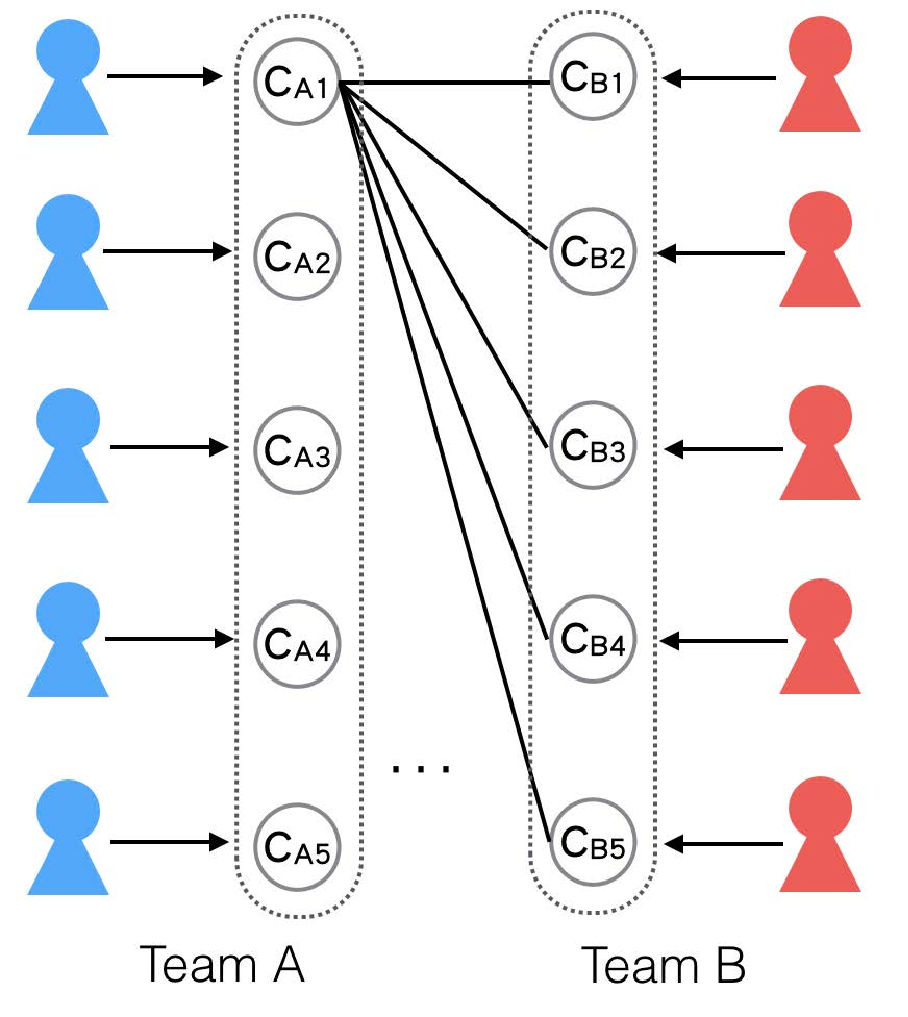
\includegraphics[width=65mm]{team_comp.pdf}
  \caption{An illustration of team composition and the aspects that may influences the game result.}
  \label{fig:team_comp}
\end{figure}

Unlike the character ranking model where we make the independent assumption between player skills and game results. The group ranking model not only considers the player skills, but also take the relationship of different characters into account. For example, Fig. \ref{fig:team_comp} has shown the factors that may have potential influence on the game result. It can be seen from the figure that the performance of one specific character should affect all the other characters in the different team. This is not difficult to understand because there are many times in the game that all the characters in a team will need to work together to achieve their goals. Therefore, to learn the team composition, we need also use such information.

To utilize these additional information, we first introduce the character matrix.
\begin{definition}
A matrix $A \in \mathbb{R}^{N\times N}$ is called the character matrix if the element $a_{i,j}$ indicates the probability that the team with character $i$ beats the team with character $j$, i.e. $a_{i,j}=\text{Pr}\{\text{team with $c_i$ beats team with $c_j$}\}$.
\end{definition}

The character matrix gives us an evaluation between different character pair that can be used for learning. However, to obtain a more complete feature we may also need to consider the impact of the players (i.e., use a function $g(P_{\mathcal{A},i},P_{\mathcal{B},j})$ to evaluate the winning ratio between two players), spo the final feature could be a matrix $F \in \mathbb{R}^{N\times N}$ based on this information. The element of feature matrix is defined as
\begin{equation}
f_{i,j}=a_{i,j} \cdot g(P_{\mathcal{A},i},P_{\mathcal{B},j}),
\end{equation}
where the $a_{i,j}$ is the element from character matrix, $g(P_{\mathcal{A},i},P_{\mathcal{B},j})$ is the function that measure the winning ratio between the player in group $\mathcal{A}$ using character $i$ and the player in group $\mathcal{B}$ using character $j$. Notice that we can multiply these two elements because they are independent.

\begin{remark}
There is no doubt that the feature matrix contains more information than the plain character feature in the character ranking model. However, one of the biggest challenge when applying the feature matrix is its high dimension (i.e. $N\times N$, which will also lead to the sparsity of the parameters). To solve this problem, we will use the clustering methods to cluster the $N$ characters into $K$ groups, so that the comparison between two individual characters will become the comparison between two clusters. Thus the dimension problem will be reduced. (This will be the one of the work during the second part of this semester.)
\end{remark}



\section{Performance Evaluation}



\begin{figure}[t]
  \centering
    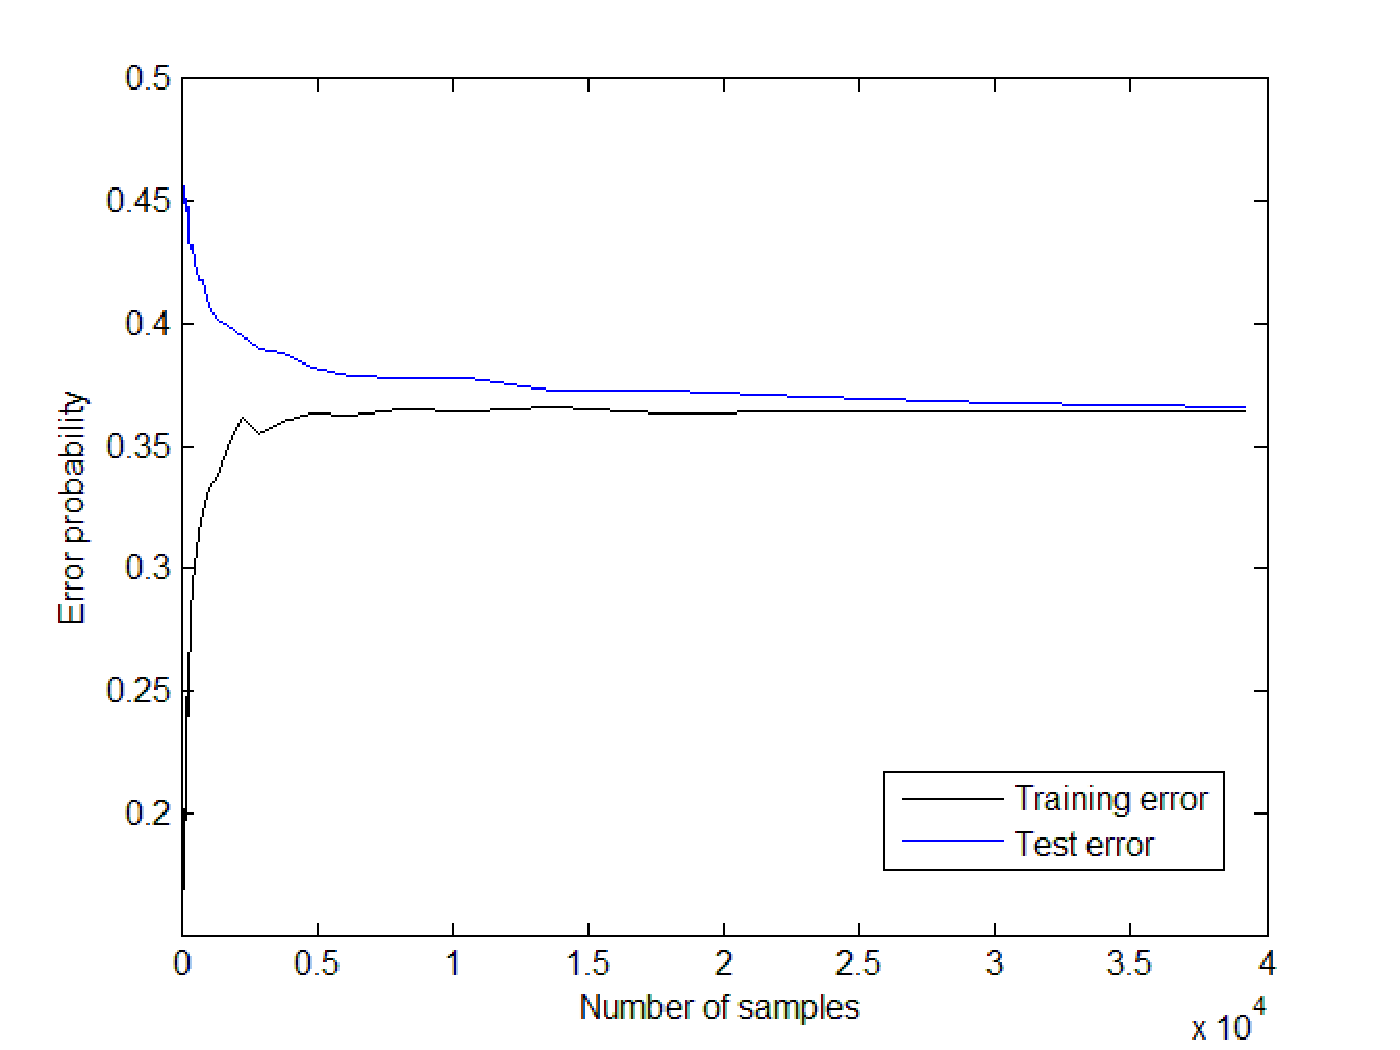
\includegraphics[width=90mm]{dota2_logreg_error.pdf}
  \caption{The error probability of logistic regression on the DotA 2 dataset.}
  \label{fig:dota2_log}
\end{figure}


\begin{figure}[t]
  \centering
    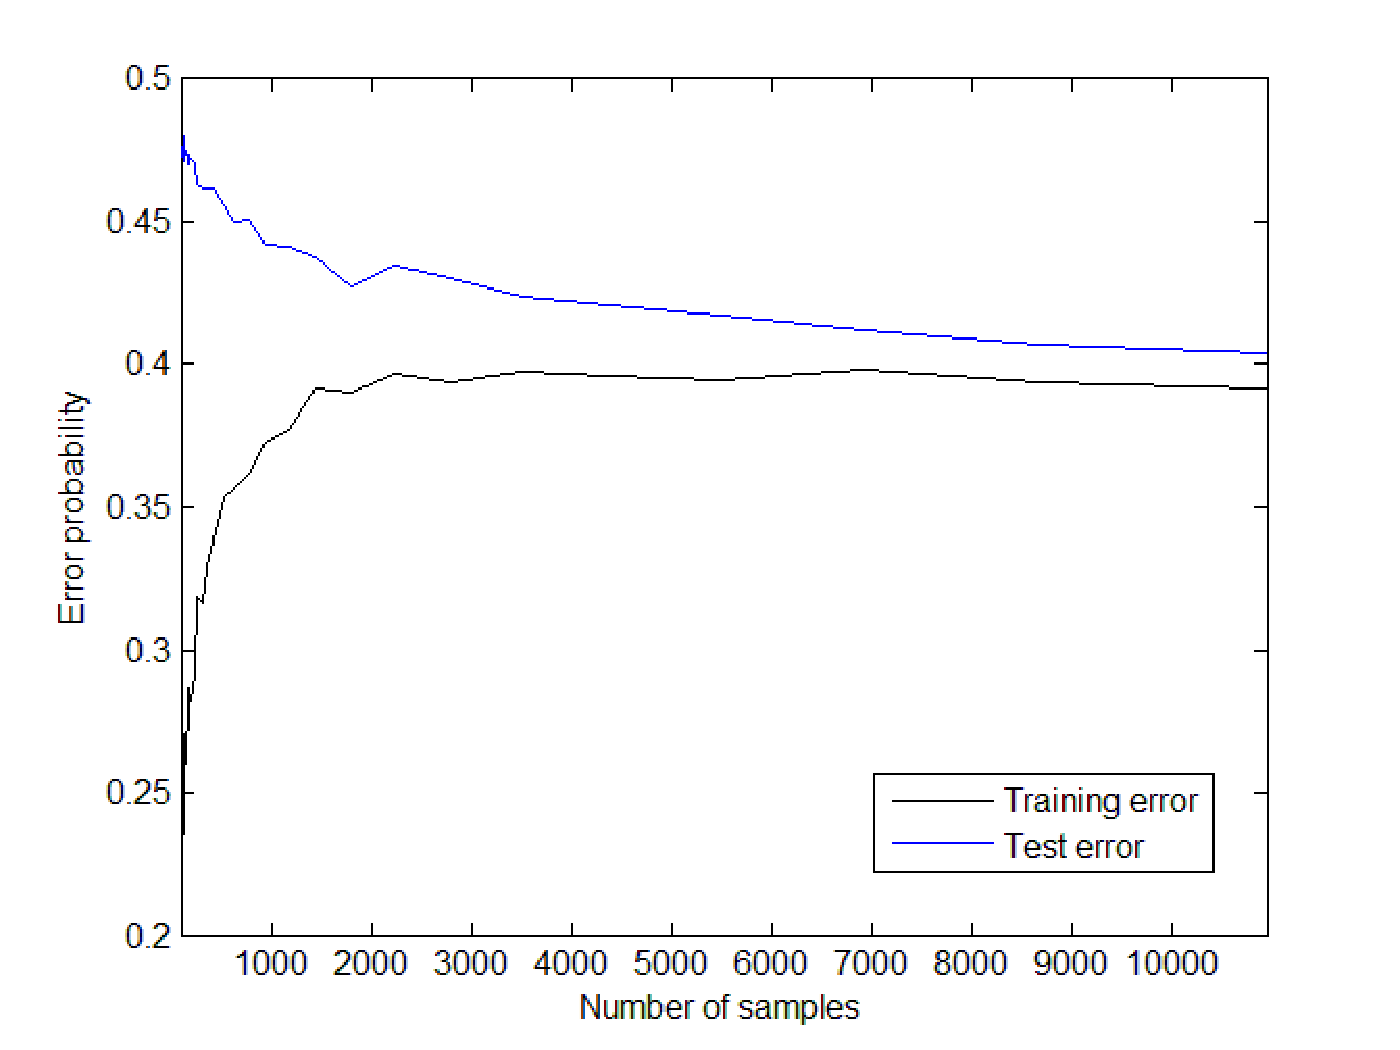
\includegraphics[width=90mm]{lol_logreg_error.pdf}
  \caption{The error probability of logistic regression on the LoL dataset.}
  \label{fig:lol_log}
\end{figure}



\subsection{Evaluation of logistic regression}

Fig. 2 and 3 show the error probability versus training sample on two dataset with Logistic Regression, We select a learning rate of $\alpha = 0.001$, the proportion of test set is 30\%, which is randomly picked from the dataset. For each data set, the iteration time for gradient decent is 100 during the training.

This figure represents the learning curve for logistic regression algorithm. With small number of training examples, we obtained a small training error and a large testing error. As we increase the number of training examples, the training error increase and testing error decreases. For DotA 2, both test error and training error converges to $36.5\%$ after around 10,000 training points.

The weight vector we obtained in logistic regression represents each character's influence on game result. For character $i$, a positive weight $w_i$ implies that picking this character will increase the chance of winning. Therefore, the prediction is based on individual characters and does not consider synergy between characters.

\subsection{Evaluation of neural network}
In neural networks model, we choose to use 3 layers: 1 hidden layer with 100 nodes. The input layer has p nodes and the output layer has 2 nodes. We implemented feedforward back propagation neural network. Sigmoid transform was applied and lambda in cost function was set to 0.5. (Since the evaluation of error probability versus the number of sample is too expensive for neural networks, we didn't do that in this midway report, but we will add it in the final report)

\subsection{Comparison of algorithms}

\begin{table}[ht]
\center
\captionsetup{font={small}}
\caption{performance of different algorithms}
\begin{tabular}{|c |c |c |c |c |}
\hline
& \multicolumn{2}{c|}{LoL}    & \multicolumn{2}{c|}{Dota 2}   \\
\hline
Accuracy (\%)                       & Training   & Test  & Training  & Test  \\ \hline
Logistic Regression    & 62.55         & 60.62     & 63.06         & 63.48     \\ \hline
Neural Networks       & 72.63        & 70.77     & 65.12        &64.81     \\ \hline
\end{tabular}
\end{table}

While we can not directly interpret the parameters we obtained from neural networks model, the high accuracy shows the importance of considering the relationship between selected characters. Since logistic regression has a linear decision boundary, it can only make prediction based on a linear combination of individual characters. Therefore, logistic regression can not capture the relationship between selected characters. On the other side, the learning process of Neural Network combines input feature in the hidden layer to take consideration of the relationship between selected characters.

\subsection{Comparison of data sets}
Logistic regression yield similar accuracy for LoL and DotA 2 while neural networks has better result on LoL than DotA 2. This result from logistic regression implies that in LoL and DotA 2, selection of individual characters have similar impact on game result. One possible explanation for higher accuracy in LoL data set when using neural networks is that the team composition in LoL focus more on the synergy between characters, thus considering more complicated relationship between characters gives better result.



\section{Conclusion and Future Work}

Team composition has been a interesting as well as challenging problem especially in the setting of competitive online games. A good team composition will strongly improve your chance for wining, while a bad team composition may probably ruin your game.

In this report, we studied the team composition in the massive online battle arena (MOBA) games, and tried to decode the impact of team composition.
During first half of the semester, we finished the goal we set in the proposal including:
\begin{itemize}
\item collect data set from LoL and DotA 2
\item build feature model
\item run logistic regression on each data set
\item run neural network on each data set
\end{itemize}

Our current results shows that the team composition does have connection with game results and the relationship is encodable. However, due to the limitation of original model, we proposed a second model to encode the relationship between selected characters and the players.

For the remaining semester, our plan is shown as follows
p
Nov 1 - Nov 15: Set up and run logistic regression and deep learning algorithm on our dataset using new model.

Nov 16 - Nov 30: Analysis our result and tune parameters for different algorithm.

To make the project successful, the minimum requirement is not longer the data collection, pre-processing and algorithms implementation, but to validate our model and make a better analysis and learn well.



% An example of a floating figure using the graphicx package.
% Note that \label must occur AFTER (or within) \caption.
% For figures, \caption should occur after the \includegraphics.
% Note that IEEEtran v1.7 and later has special internal code that
% is designed to preserve the operation of \label within \caption
% even when the captionsoff option is in effect. However, because
% of issues like this, it may be the safest practice to put all your
% \label just after \caption rather than within \caption{}.
%
% Reminder: the "draftcls" or "draftclsnofoot", not "draft", class
% option should be used if it is desired that the figures are to be
% displayed while in draft mode.
%
%\begin{figure}[!t]
%\centering
%\includegraphics[width=2.5in]{myfigure}
% where an .eps filename suffix will be assumed under latex,
% and a .pdf suffix will be assumed for pdflatex; or what has been declared
% via \DeclareGraphicsExtensions.
%\caption{Simulation Results}
%\label{fig_sim}
%\end{figure}

% Note that IEEE typically puts floats only at the top, even when this
% results in a large percentage of a column being occupied by floats.


% An example of a double column floating figure using two subfigures.
% (The subfig.sty package must be loaded for this to work.)
% The subfigure \label commands are set within each subfloat command, the
% \label for the overall figure must come after \caption.
% \hfil must be used as a separator to get equal spacing.
% The subfigure.sty package works much the same way, except \subfigure is
% used instead of \subfloat.
%
%\begin{figure*}[!t]
%\centerline{\subfloat[Case I]\includegraphics[width=2.5in]{subfigcase1}%
%\label{fig_first_case}}
%\hfil
%\subfloat[Case II]{\includegraphics[width=2.5in]{subfigcase2}%
%\label{fig_second_case}}}
%\caption{Simulation results}
%\label{fig_sim}
%\end{figure*}
%
% Note that often IEEE papers with subfigures do not employ subfigure
% captions (using the optional argument to \subfloat), but instead will
% reference/describe all of them (a), (b), etc., within the main caption.


% An example of a floating table. Note that, for IEEE style tables, the
% \caption command should come BEFORE the table. Table text will default to
% \footnotesize as IEEE normally uses this smaller font for tables.
% The \label must come after \caption as always.
%
%\begin{table}[!t]
%% increase table row spacing, adjust to taste
%\renewcommand{\arraystretch}{1.3}
% if using array.sty, it might be a good idea to tweak the value of
% \extrarowheight as needed to properly center the text within the cells
%\caption{An Example of a Table}
%\label{table_example}
%\centering
%% Some packages, such as MDW tools, offer better commands for making tables
%% than the plain LaTeX2e tabular which is used here.
%\begin{tabular}{|c||c|}
%\hline
%One & Two\\
%\hline
%Three & Four\\
%\hline
%\end{tabular}
%\end{table}


% Note that IEEE does not put floats in the very first column - or typically
% anywhere on the first page for that matter. Also, in-text middle ("here")
% positioning is not used. Most IEEE journals/conferences use top floats
% exclusively. Note that, LaTeX2e, unlike IEEE journals/conferences, places
% footnotes above bottom floats. This can be corrected via the \fnbelowfloat
% command of the stfloats package.



%\section{Conclusion}
%The conclusion goes here.




% conference papers do not normally have an appendix


% use section* for acknowledgement
%\section*{Acknowledgment}


%The authors would like to thank...





%p trigger a \newpage just before the given reference
% number - used to balance the columns on the last page
% adjust value as needed - may need to be readjusted if
% the document is modified later
%\IEEEtriggeratref{8}
% The "triggered" command can be changed if desired:
%\IEEEtriggercmd{\enlargethispage{-5in}}

% references section

% can use a bibliography generated by BibTeX as a .bbl file
% BibTeX documentation can be easily obtained at:
% http://www.ctan.org/tex-archive/biblio/bibtex/contrib/doc/
% The IEEEtran BibTeX style support page is at:
% http://www.michaelshell.org/tex/ieeetran/bibtex/
%\bibliographystyle{IEEEtran}
% argument is your BibTeX string definitions and bibliography database(s)
%\bibliography{IEEEabrv,../bib/paper}
%
% <OR> manually copy in the resultant .bbl file
% set second argument of \begin to the number of references
% (used to reserve space for the reference number labels box)


\begin{thebibliography}{10}

\bibitem{Ian}
Ian Sherr, ``Player Tally for League of Legends Surges,'' \textit{Digits RSS. N.p., n.d. Web}. 28 Sept, 2014.

\bibitem{Valve}
Valve, Dota 2 -- 2014 Compendium -- The International. Dota 2 Official Website.

\end{thebibliography}




% that's all folks
\end{document}

%\begin{table}[th]\label{Tab:data_content}
%\centering
%\begin{tabular}{|c|c|}
%\hline
%Content & Description \\
%\hline
%Game ID &  \\
%\hline
%Game Duration & . \\
%\hline
%Winner &  \\
%\hline
% Upper Adjacent & -17 \\
%\hline
%Digital TV & Lower Adjacent
%\end{tabular}
%\end{table}
